\chapter{Funktionstest/Validierung}\label{chap:Funktionstest}
\thispagestyle{standard}
\pagestyle{standard}
\lfoot{\small Refik Kerimi}

\section{Ausgangsbedingung und Ausgrenzung}
Getestet wurden die in Kapitel \ref{chab:Basistechnologien} und \ref{chab:Implementierung} beschriebenen PWA-Features. Dies wurde zum einen über die DevTools vom Chrome Browser sowie über das Chrome PlugIN Lighthouse getestet. 
Als mobiles Testgerät wurde das Nexus X5 mit der Android 8.1.0 Software verwendet.  
Weiters kann der Emulator von Android Studio verwendet werden um den Test ohne Androidgerät darzustellen. Die Applikation selbst wurde hier nicht behandelt.
 
\section{Testen auf Mobilen Geräten und Android Studio Emulator}
Um auf auf dem Mobilen Smartphone testen zu können muss der Developer Modus auf dem Gerät eingeschaltet werden. Dies wird durch das Aktivieren der Entwicklertools und das Freischalten der USB-Debugging Funktion wie in Abbildung \ref{fig:DevToolsAndorid} und \ref{fig:DevToolsChrome} zu sehen ist erreicht. 

\begin{figure}[h]
	\centering
	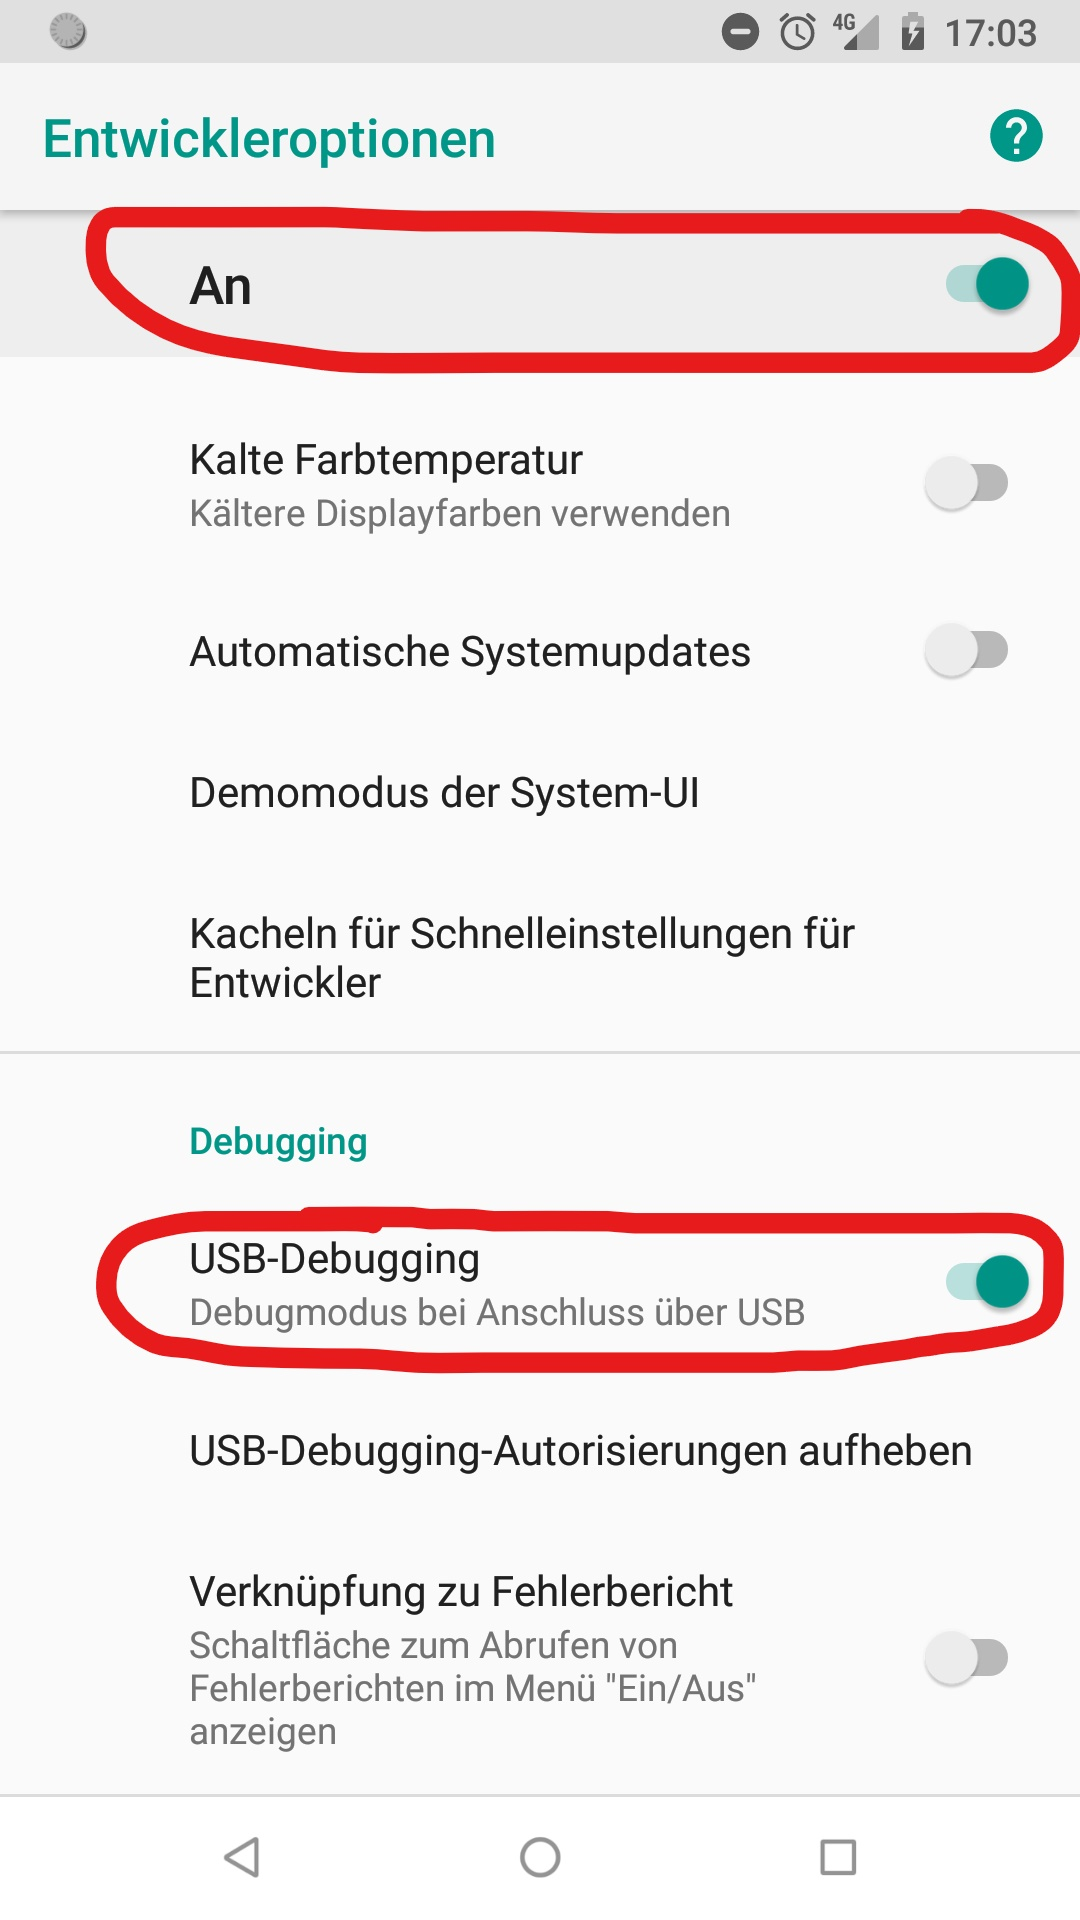
\includegraphics[width=6cm]{BilderAllgemein/DevToolsAndroid}\medskip
	\caption{Aktivieren der Entwicklertools auf Android 8.1.0}
	\label{fig:DevToolsAndorid}
\end{figure}

\begin{figure}[h]
	\centering
	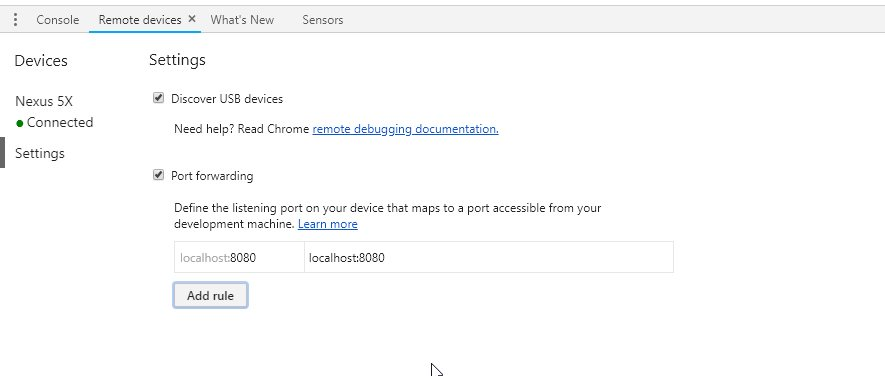
\includegraphics[width=14cm]{BilderAllgemein/DevToolsChrome}\medskip
	\caption{Anzeige der Verbindung auf Google Chrome 67}
	\label{fig:DevToolsChrome}
\end{figure}
\newpage
Falls kein Android Gerät zur Verfügung steht ist der von Android Studio\footnote{https://developer.android.com/studio/} angebotene Emulator eine große Hilfe. Durch den integrierten Emulator lassen sich verschiedene Softwareversionen von Android darstellen. Sie helfen bei der Entwicklung und beim Testen der \acs{PWA}.

\section{Lighthouse}
Lighthouse ist ein open-source Tool von Google und unterstützt den Entwickler bei der Verbesserung und Transformation der Applikation zu einer vollwärtigen \acs{PWA}. Man kann Lighthouse über 3 Wege verwenden:
\begin{itemize}
    \item  in Chrome DevTools
	\item  über die Kommandozeile
	\item  oder im Continues Integration Prozess als Node Module
\end{itemize}
Jeder dieser Workflows benötigt den Google Chrome Browser \cite{Lighthouse}.



\section{Add to Homescreen}
%https://developers.google.com/web/fundamentals/app-install-banners/#test


\section{Service Worker}



\section{Push Notifikation}



\section{Geolocation}


\section{Vergleich mit native App}
Verglichen wurden die Punkte wie Kapitel \ref{chap:UnterschiedePWA,NativeApplikationundWeb-Apps} verwendet:
\begin{itemize}
   \item   Installation
	\item  Zugriff
	\item  Funktionen
\end{itemize}. 





